\documentclass{article}    

\usepackage{graphicx}

\begin{document}

% ------------------------------------------ figure 4

\begin{figure}[!t] \centering
  \begin{tabular}{ccc}
    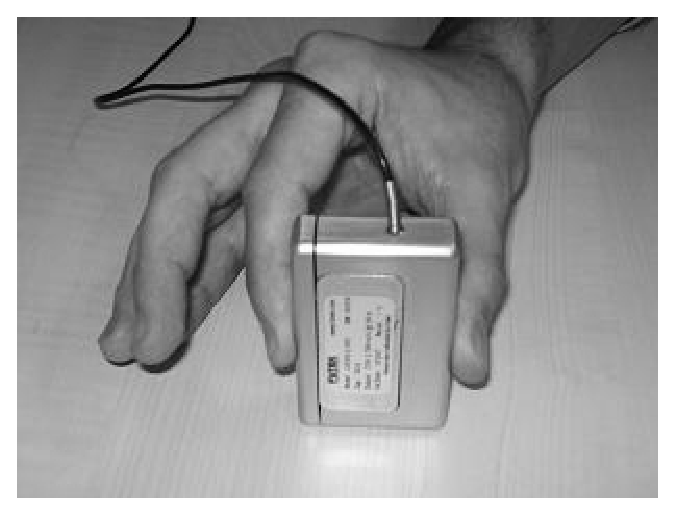
\includegraphics[width=0.30\textwidth]{grip1.eps} &
    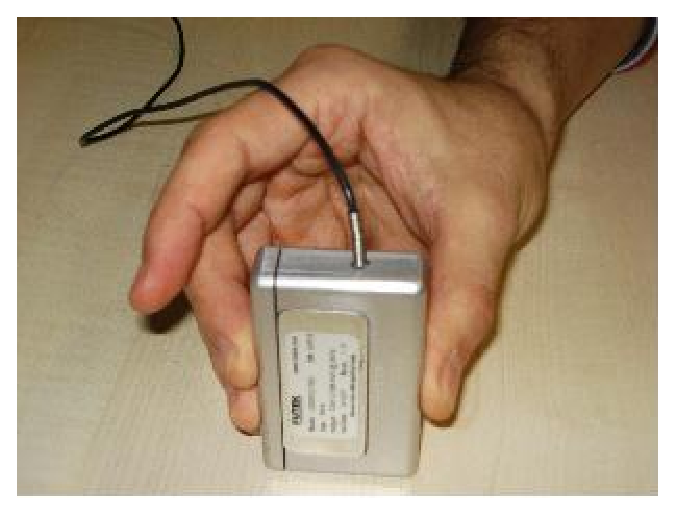
\includegraphics[width=0.30\textwidth]{grip2.eps} &
    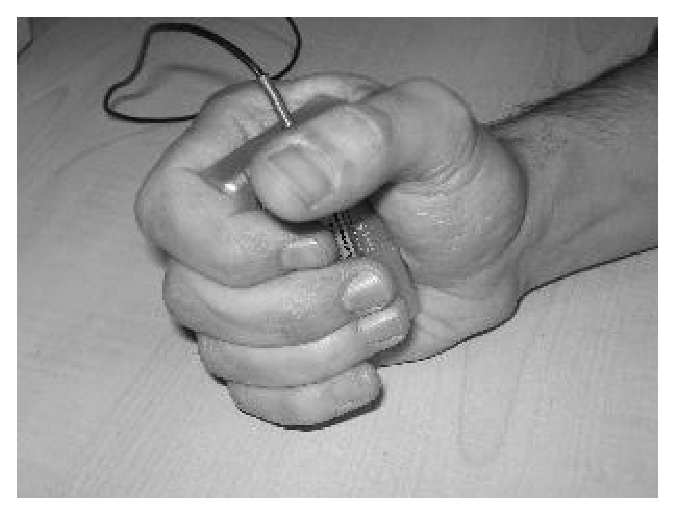
\includegraphics[width=0.30\textwidth]{grip3.eps} \\
    $(a)$ & $(b)$ & $(c)$ \\
  \end{tabular}
%  \caption{The three different grips employed in the experiment: $(a)$
%   index precision grip; $(b)$ other fingers precision grip; $(c)$
%   power grasp.}
%  \label{fig:Grasps}
\end{figure}

\end{document}
